\documentclass[11pt]{article}

\usepackage[a4paper,margin=1in]{geometry}
\usepackage{amsmath,amssymb}
\usepackage{booktabs,longtable,array}
\usepackage{xcolor}
\usepackage{hyperref}
\usepackage{float}
\usepackage{tikz}
\usepackage[most]{tcolorbox}
\usepackage{listings}
\usepackage{enumitem}
\usetikzlibrary{arrows.meta,positioning}

\definecolor{DeepBlue}{RGB}{18,45,74}
\definecolor{SoftBlue}{RGB}{44,112,173}
\definecolor{SoftRed}{RGB}{180,35,35}
\definecolor{DarkGreen}{RGB}{35,105,75}
\definecolor{LightGray}{RGB}{245,247,250}

\hypersetup{
  colorlinks=true,
  linkcolor=DeepBlue,
  urlcolor=SoftBlue,
  citecolor=DarkGreen
}

\newtcolorbox{importantbox}[1]{
  colback=LightGray,
  colframe=DeepBlue,
  title=\textbf{#1},
  boxrule=0.8pt,
  arc=1mm
}

\newtcolorbox{warningbox}[1]{
  colback=red!3,
  colframe=SoftRed,
  title=\textbf{#1},
  boxrule=0.8pt,
  arc=1mm
}

\lstset{
  basicstyle=\ttfamily\small,
  frame=single,
  breaklines=true,
  columns=fullflexible,
  backgroundcolor=\color{LightGray},
  rulecolor=\color{SoftBlue}
}

\title{Explanation of the Single-File Hybrid Hammerstein--LSTM Code}
\author{Hussein Zolfaghari}
\date{}

\begin{document}

\maketitle
\tableofcontents
\newpage

\section{What to run}

There is only one Python code file:

\begin{center}
\texttt{Hybrid\_Hammerstein\_LSTM\_VSCode.py}
\end{center}

Place the Python file and \texttt{COMSOL\_07\_13\_2026.xlsx} in the same folder. Open the Python file in Visual Studio Code and click \emph{Run Python File}. No batch file and no Windows Command Prompt are required.

The Python file automatically checks whether NumPy, Matplotlib, OpenPyXL, and PyTorch are available. Missing packages are installed using the same Python interpreter selected in Visual Studio Code.

\section{Data usage}

The code reads five worksheets directly from the supplied Excel workbook.

\begin{table}[H]
\centering
\begin{tabular}{ll}
\toprule
Purpose & Worksheets \\
\midrule
Training and validation &
67, 87, 107, and 127\,mA \\
Independent test &
147\,mA \\
\bottomrule
\end{tabular}
\end{table}

The 147\,mA record is never used for normalization, training, validation, or model selection.

The four development records are divided into complete non-overlapping time blocks. Approximately 80\% of the blocks are randomly assigned to training and 20\% to validation. This approach is preferred to randomly splitting individual overlapping windows because adjacent windows share nearly all of their samples.

\section{Input and output variables}

The known model inputs are:

\[
u(k)=
\begin{bmatrix}
I(k) &
\Delta I(k) &
I_{\mathrm{DC}}
\end{bmatrix}^{T},
\]

where $I(k)$ is coil current, $\Delta I(k)$ is the current increment, and $I_{\mathrm{DC}}$ identifies the operating offset.

The measured outputs are:

\[
y(k)=
\begin{bmatrix}
x(k) &
F(k)
\end{bmatrix}^{T},
\]

where $x$ is displacement and $F$ is Lorentz force.

The model uses the previous 120 samples to predict the next output.

\section{Ogunmolu/Gans contribution}

Ogunmolu et al.\ studied neural architectures for nonlinear dynamic-system identification and implemented feedforward, recurrent, LSTM, FastLSTM, and GRU paths in the FARNN repository \cite{ogunmolu2016,farnnrepo}.

A classical Hammerstein structure separates a static nonlinearity from a dynamic block:

\begin{align}
v(k)&=g(u(k)),\\
\hat y(k)&=G(q^{-1})v(k).
\end{align}

The present code adapts this concept as:

\[
u(k)
\xrightarrow{\text{static neural nonlinearity}}
v(k)
\xrightarrow{\text{LSTM dynamics}}
\hat y(k+1).
\]

The static block is:

\begin{lstlisting}[language=Python]
self.static_nonlinearity = nn.Sequential(
    nn.Linear(3, STATIC_SIZE),
    nn.Tanh(),
    nn.Linear(STATIC_SIZE, STATIC_SIZE),
    nn.Tanh(),
)
\end{lstlisting}

The dynamic block is:

\begin{lstlisting}[language=Python]
self.lstm = nn.LSTM(
    input_size=STATIC_SIZE + 2,
    hidden_size=HIDDEN_SIZE,
    batch_first=True,
)
\end{lstlisting}

The additional two LSTM inputs are the historical displacement and force.

\begin{importantbox}{Relationship to the GitHub repository}
The code is a PyTorch adaptation of the modeling idea. It is not a line-by-line conversion or direct import of the original Lua/Torch7 FARNN source.
\end{importantbox}

\section{Wang contribution}

\subsection{Series--parallel training}

Wang's series--parallel identifier uses measured past outputs:

\[
\hat y(k)
=
F\!\left(
u_{\mathrm{past}},
y_{\mathrm{past}}
\right).
\]

The first training stage in the code follows this structure. Every input window includes measured historical displacement and force.

This stage is stable because the model does not initially depend on its own previous errors.

\subsection{Scheduled recursive training}

The earlier implementation trained only with measured outputs and switched suddenly to predicted feedback during free-running testing. This caused error accumulation.

The new code adds a second training stage. The feedback is selected as:

\[
y_{\mathrm{feedback}}(k)=
\begin{cases}
y(k), & \text{with probability }p,\\
\hat y(k), & \text{with probability }1-p.
\end{cases}
\]

The probability $p$ gradually decreases from approximately 0.9 to 0.1. Therefore, the model learns to operate with its own predictions.

The recursive training loss includes all steps of a short horizon:

\[
\mathcal{L}_{\mathrm{rollout}}
=
\frac{1}{BK}
\sum_{b=1}^{B}
\sum_{j=1}^{K}
\left\|
y_b(k+j)-\hat y_b(k+j)
\right\|^2.
\]

\subsection{What is not copied from Wang}

Wang also combines several LSTM estimators through adaptive convex coefficients:

\[
\hat y(k)
=
\sum_{i=1}^{N}
\alpha_i(k)\hat y_i(k).
\]

The present code intentionally uses one LSTM so that the implementation remains understandable.

\section{Complete model}

\begin{figure}[H]
\centering
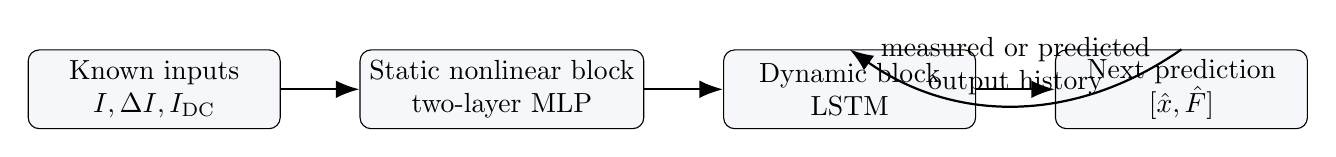
\begin{tikzpicture}[
node distance=1.0cm and 1.0cm,
box/.style={
draw,
rounded corners,
minimum width=3.2cm,
minimum height=1cm,
align=center,
fill=LightGray
},
arrow/.style={-{Latex[length=3mm]},thick}
]
\node[box] (input) {Known inputs\\$I,\Delta I,I_{\mathrm{DC}}$};
\node[box,right=of input] (static) {Static nonlinear block\\two-layer MLP};
\node[box,right=of static] (lstm) {Dynamic block\\LSTM};
\node[box,right=of lstm] (output) {Next prediction\\$[\hat x,\hat F]$};

\draw[arrow] (input) -- (static);
\draw[arrow] (static) -- (lstm);
\draw[arrow] (lstm) -- (output);
\draw[arrow,bend left=35]
(output.north) to node[above,align=center]
{measured or predicted\\output history} (lstm.north);
\end{tikzpicture}
\caption{Hybrid Hammerstein--LSTM model}
\end{figure}

The output layer predicts the change from the most recent output:

\[
\hat y(k+1)
=
y_{\mathrm{history}}(k)
+
\Delta\hat y(k+1).
\]

This residual form is used to improve numerical stability and reduce drift.

\section{Training process}

The code performs the following steps:

\begin{enumerate}[leftmargin=*]
\item Read the five worksheets.
\item Randomly assign development blocks to training or validation.
\item Calculate normalization statistics from training blocks only.
\item Create 120-sample input windows.
\item Train the model in series--parallel mode.
\item Fine-tune the model using scheduled recursive prediction.
\item Predict the complete unseen 147\,mA dataset.
\item Evaluate one-step and parallel/free-running predictions.
\item Save figures, numerical tables, model weights, and settings.
\end{enumerate}

The one-step cost is normalized mean squared error:

\[
\mathcal{L}_{1}
=
\frac{1}{B}
\sum_{b=1}^{B}
\left\|
y_b(k+1)
-
\hat y_b(k+1)
\right\|^2.
\]

\section{Generated outputs}

Each run creates one timestamped subfolder inside each of the following folders:

\begin{itemize}[leftmargin=*]
\item \texttt{01\_Report\_Figures};
\item \texttt{02\_Presentation\_Figures};
\item \texttt{03\_Complete\_Results}.
\end{itemize}

The code saves:

\begin{itemize}[leftmargin=*]
\item training and validation cost functions;
\item the random block assignment figure;
\item complete measured-versus-predicted displacement;
\item complete measured-versus-predicted Lorentz force;
\item one-step and parallel prediction errors;
\item parity plots;
\item an accuracy table;
\item \texttt{test\_metrics.csv};
\item \texttt{training\_history.csv};
\item \texttt{147mA\_full\_predictions.csv};
\item the trained PyTorch model.
\end{itemize}

Accuracy is reported using MSE, RMSE, MAE, $R^2$, and fit percentage.

\section{Important limitation}

\begin{warningbox}{Accuracy must be determined by the full run}
The revised structure is designed to reduce recursive error, but no honest implementation can guarantee a specific accuracy before completing the full training. The final judgment must use both one-step and parallel metrics in \texttt{test\_metrics.csv}.
\end{warningbox}

The 147\,mA dataset is an extrapolation because the development offsets end at 127\,mA. Its result is therefore a more difficult and more meaningful test than interpolation within the development range.

\section{Settings that may be changed}

The main settings are near the beginning of the Python file:

\begin{lstlisting}[language=Python]
WINDOW = 120
HIDDEN_SIZE = 64
STATIC_SIZE = 24
ONE_STEP_EPOCHS = 30
ROLLOUT_EPOCHS = 12
ROLLOUT_HORIZON = 12
\end{lstlisting}

Use the original settings for the first complete run. Changes should be made only after reviewing the training, validation, and independent-test results.

\section{Summary}

The single Python file now contains the complete workflow requested:

\begin{itemize}[leftmargin=*]
\item four development datasets and one unseen test dataset;
\item random non-overlapping training and validation blocks;
\item PyTorch neural-network implementation;
\item explicit Hammerstein-type static nonlinearity;
\item LSTM dynamic modeling;
\item Wang series--parallel training;
\item scheduled recursive multi-step training;
\item complete test-record prediction;
\item cost, accuracy, prediction, and error figures;
\item report, presentation, and complete-result folders.
\end{itemize}

\begin{thebibliography}{9}

\bibitem{wang2017}
Y. Wang,
``A New Concept using LSTM Neural Networks for Dynamic System Identification,''
\emph{Proceedings of the 2017 American Control Conference},
Seattle, WA, 2017, pp.~5324--5329.

\bibitem{ogunmolu2016}
O. Ogunmolu, X. Gu, S. Jiang, and N. Gans,
``Nonlinear Systems Identification Using Deep Dynamic Neural Networks,''
arXiv:1610.01439, 2016.

\bibitem{farnnrepo}
O. Ogunmolu,
``FARNN: Fully Automated Recurrent Neural Network for Dynamic System Identification,''
GitHub repository,
\url{https://github.com/robotsorcerer/FARNN}.

\end{thebibliography}

\end{document}
